% =====================================================================================
%  supplementary_1.tex — Matériel supplémentaire de l'article de conférence (révision 1)
%  Contient tout ce qui a été retiré du corps pour respecter la limite de 6 pages :
%   S1 Nomenclature complète (reclassée selon le commentaire R10)
%   S2 Modèle détaillé (anciennes Éq. 4–7, Fig. 1 circuit, Fig. 2 BEopt, architecture)
%   S3 Identification (cadre EKF, protocole, identifiabilité, Tableau II)
%   S4 Preuve de la Proposition 1 et variante stricte
%   S5 Paramètres complets (ancien Tableau IV)
%   S6 Résultats complémentaires (Fig. J3 à 4 panneaux, variante stricte, équité, robustesse)
%  Notation identique à main_1.tex. Compiler avec pdflatex + bibtex (même refs_1.bib).
% =====================================================================================
\documentclass[10pt,letterpaper]{article}
\usepackage[margin=0.9in]{geometry}
\usepackage[T1]{fontenc}
\usepackage[utf8]{inputenc}
\usepackage{mathptmx}                     % police Times proche d IEEEtran
\usepackage{amsmath,amssymb}
\usepackage{graphicx}\graphicspath{{figures/}}
\usepackage{booktabs,array,longtable}
\usepackage{caption}
\usepackage[hidelinks]{hyperref}
\usepackage{cite}
\usepackage{newunicodechar}
\newunicodechar{≈}{\ensuremath{\approx}}\newunicodechar{≤}{\ensuremath{\leq}}\newunicodechar{≥}{\ensuremath{\geq}}
\newunicodechar{→}{\ensuremath{\rightarrow}}\newunicodechar{−}{\ensuremath{-}}
\newcommand{\Penv}{P_{\mathrm{env}}}
\newcommand{\PB}{P_{\mathrm{B}}}
% numérotation propre au supplément : S1, S2… ; Fig. S1… ; Table S1… ; Éq. (S1)…
\renewcommand{\thesection}{S\arabic{section}}
\renewcommand{\thefigure}{S\arabic{figure}}
\renewcommand{\thetable}{S\arabic{table}}
\renewcommand{\theequation}{S\arabic{equation}}

\title{\textbf{Supplementary Material}\\[2pt]\large Predictive Coordination of Building Thermal Mass and Electric Thermal Storage in a Multi-Unit Residential Building to Relieve a Distribution Transformer during Winter Peaks}
\author{D. A. Anyouzo'o, N. Henao, D. Toquica, K. Agbossou, F. Kloutse, O. T. Sosso, A. Parrado Duque}
\date{}

\begin{document}
\maketitle
\noindent Equation, figure and table numbers without the prefix ``S'' refer to the main paper.

% -------------------------------------------------------------------------------------
\section{Nomenclature}\label{s:nom}
% [R10] Classement demandé : Acronyms, Indices, Sets, Parameters, Variables.
{\small
\begin{longtable}{@{}>{\raggedright\arraybackslash}p{0.24\linewidth}>{\raggedright\arraybackslash}p{0.70\linewidth}@{}}
\multicolumn{2}{@{}l}{\textbf{Acronyms}}\\
ADMM & Alternating direction method of multipliers \\
COP & Coefficient of performance \\
DTR & Dynamic thermal rating \\
EKF & Extended Kalman filter \\
ETS & Electric thermal storage (refractory-brick unit) \\
EV & Electric vehicle \\
FCI & Flexibility contribution index \\
HEMS & Home energy management system \\
HP & Heat pump \\
LoL & Loss of life \\
MPC & Model predictive control \\
MUB & Multi-unit residential building \\
NIS & Normalized innovation squared \\
ONAN & Oil natural, air natural (transformer cooling) \\
PF & Power factor \\
PID & Proportional-integral-derivative (controller) \\
PRBS & Pseudo-random binary sequence \\
SLSQP & Sequential least-squares quadratic programming \\
SOC & State of charge \\[4pt]
\multicolumn{2}{@{}l}{\textbf{Indices}}\\
$n$, $n'$, $l$ & Dwelling; adjacent dwelling; generic dwelling in sums \\
$p$ & Floor \\
$t$ & Time step (sampling period $\Delta t$) \\
$j$ & Step within the prediction horizon \\[4pt]
\multicolumn{2}{@{}l}{\textbf{Sets}}\\
$\mathcal A_n$ & Dwellings adjacent to dwelling $n$ \\
$\mathcal N_p$ & Dwellings of floor $p$ \\
$\mathcal C$, $\mathcal C_{\sigma+}$ & Congestion set; next congestion after period $\sigma$ \\
$\sigma$ & Off-congestion period \\[4pt]
\multicolumn{2}{@{}l}{\textbf{Parameters}}\\
$S_n$, $K_s$, $P_{lim}$ & Transformer rated power (kVA); safety margin; active-power limit $(1-K_s)S_n\mathrm{PF}$ (kW) \\
$R_L$ & Ratio of load to no-load losses \\
$\Delta\theta_{TO,R}$, $\Delta\theta_{H,R}$ & Rated top-oil and hot-spot rises (K) \\
$\tau_{TO}$, $\tau_w$ & Oil and winding time constants \\
$x$, $y$ & Oil and winding exponents \\
$C_i$, $C_e$, $C_c$, $C_s$ & Heat capacities of air, envelope, ETS core and casing (J/K) \\
$m_c$, $c_p$ & Brick mass (kg); specific heat (J/(kg·K)) \\
$R_i$, $R_o$ & Air--envelope and envelope--outdoor resistances (K/W) \\
$R_{nn'}$, $R_h$ & Resistances to the adjacent dwelling and to the corridor (K/W) \\
$R_c$, $R_s$, $R_{conv,\min}$ & ETS core--casing, casing--air and minimum forced-convection resistances (K/W) \\
$\alpha$ & Outdoor weight of the corridor temperature \\
$A_s$, $Q_0$ & Equivalent solar aperture (m²); identified unmeasured internal gain (W) \\
$T_{c,\min}$, $T_{c,\max}$ & ETS core temperature bounds (°C) \\
$P_{h,\max}$, $P_{ETS,\max}$, $Q_{ETS,\max}$ & HP and ETS power limits (kW) \\
$T_d$, $\Delta T_n$ & Daytime setpoint; night setback (°C) \\
$\Delta_{pre}$, $\Delta_{eff}$, $\delta$ & Preheating offset; peak setback; comfort tolerance (°C) \\
$J_{pre}$, $J_{rep}$, $\tau_{min}$ & Preheating and recovery durations; minimum congestion duration \\
$w_L$, $w_T$, $\kappa$, $\lambda_{pl}$ & Weights, steepness and floor cost of the scarcity index \\
$s$, $f_b$, $W_{\max}$ & Envelope sizing factor; recharge margin; usable ETS capacity \\
$\mathrm{SOC}_{tgt}$ & Target state of charge \\
$\gamma_n$, $G_n$ & Fixed share; conductance to unheated zones \\
$H$, $\mu_c$, $\mu_b$, $\mu_h$, $\mu_\Delta$, $\mu_T$ & MPC horizon (steps) and weights \\[4pt]
\multicolumn{2}{@{}l}{\textbf{Variables}}\\
$K$ & Transformer load factor $S/S_n$ \\
$\theta_a$, $\theta_{TO}$, $\theta_{TO,u}$, $\theta_{HS}$ & Ambient, top-oil, ultimate top-oil and hot-spot temperatures (°C) \\
$F_{AA}$ & Aging acceleration factor \\
$T_i$, $T_e$, $T_{ext}$, $T_{h,p}$ & Indoor-air, envelope, outdoor and corridor temperatures (°C) \\
$T_c$, $T_s$ & ETS core and casing temperatures (°C) \\
$P_h$, $P_{ETS}$, $Q_{ETS}$ & HP electric power; ETS charging power; ETS heat release (W) \\
$Q_{int}$, $I_{gh}$ & Occupancy gains (W); global horizontal irradiance (W/m²) \\
$\beta$, $\xi$ & Log-parameters; EKF augmented state \\
$\PB$, $P_{nf}$, $P_{coord}$ & Reference load (S0); non-flexible load (base + EV); coordinated load (S1) \\
$P_{h,n,\mathrm B}$, $\theta_{HS,\mathrm B}$ & HP power and hot-spot temperature of the reference \\
$\Penv$, $L_\sigma$, $W_\sigma$ & Dynamic envelope; valley-filling level; required recharge energy \\
$M$, $c_n$, $\gamma_{r,n}$ & Building recharge margin; power cap of agent $n$; dynamic recharge share \\
$\lambda$, $\tilde\lambda$ & Scarcity index; index plus floor cost \\
$T_{ref}$, $T_{set}$, $T_{min}$, $T_{max}$ & Reference and effective setpoints; comfort floor and upper bound \\
$U_n$ & Input sequence of agent $n$ over the horizon \\
\end{longtable}}

% -------------------------------------------------------------------------------------
\section{Detailed Dwelling, Storage and Architecture Models}\label{s:model}
% [R30] Développement complet retiré du corps (anciennes Éq. 4–7).
Each dwelling $n$ is coupled to its adjacent dwellings $n'\in\mathcal A_n$, to the corridor of its floor and to its ETS (Fig.~\ref{fig:s-rc}) \cite{Bacher2011, Belic2021}. The envelope node obeys
\begin{equation}
C_{e,n}\dot T_{e,n}=\frac{T_{ext}-T_{e,n}}{R_{o,n}}+\frac{T_{i,n}-T_{e,n}}{R_{i,n}},
\end{equation}
the indoor-air node obeys Eq.~(4) of the paper, and the ETS core and casing obey
\begin{equation}
C_{c,n}\dot T_{c,n}=P_{ETS,n}-Q_{ETS,n}-\frac{T_{c,n}-T_{s,n}}{R_{c,n}},\qquad
C_{s,n}\dot T_{s,n}=\frac{T_{c,n}-T_{s,n}}{R_{c,n}}-\frac{T_{s,n}-T_{i,n}}{R_{s,n}},
\end{equation}
with $C_{c,n}=m_cc_p$. The corridor of floor $p$ is algebraic:
\begin{equation}
T_{h,p}=\alpha T_{ext}+\frac{1-\alpha}{|\mathcal N_p|}\sum_{n'\in\mathcal N_p}T_{i,n'}.
\end{equation}
The controlled discharge $Q_{ETS,n}$ is bounded by Eq.~(5) of the paper; evaluating the bound at the current state keeps the MPC problem convex \cite{Guzman2015, Devia2021}. Collecting these balances gives the matrices $A$, $B$, $E$ of $\dot x_n=Ax_n+Bu_n+Ed_n$, discretized exactly by Eq.~(6) \cite{VanLoan1978}.

\begin{figure}[h]
\centering
\includegraphics[width=0.55\linewidth]{fig1_rc.png}
\caption{Coupled RC model of a dwelling (4R2C) and its ETS (2R2C + controlled discharge). Dwelling nodes: air $T_{i,n}$ and envelope $T_{e,n}$; ETS nodes: core $T_c$ and casing $T_s$; controlled discharge through $R_{conv}$. Branches $R_{nn'}$ and $R_{h,n}$ connect the dwelling to its neighbor and to the corridor.}
\label{fig:s-rc}
\end{figure}

\begin{figure}[h]
\centering
\includegraphics[width=0.55\linewidth]{fig2_beopt.jpg}
\caption{3D view of the BEopt digital twin of the 16-unit MUB, distributed over four floors.}
\label{fig:s-beopt}
\end{figure}

\begin{figure}[h]
\centering
\includegraphics[width=0.6\linewidth]{fig5_arch.pdf}
\caption{Two-layer architecture: the aggregator, at the transformer, broadcasts the index $\lambda(t)$ and the power cap $c_n(t)$ to the HEMS agent of each dwelling and floor; EV charging remains uncoordinated.}
\label{fig:s-arch}
\end{figure}

% -------------------------------------------------------------------------------------
\section{Identification of the Thermal Parameters}\label{s:ident}
\textbf{Data.} The data come from a BEopt 2.8.0 digital twin (Standard mode, new construction, multi-family) \cite{BEopt28} built on EnergyPlus \cite{Crawley2001}, with the 2011--2025 TMYx weather file of Trois-Rivières \cite{OneBuilding2025}. For each dwelling, two one-month experiments are simulated (January, hourly): $\mathcal E_1$, a PRBS setpoint excitation (pulsed reheats to 25 °C followed by free decays), and $\mathcal E_2$, free-floating.

\textbf{Identification model.} Identification is decoupled: neighbor and corridor temperatures are measured inputs \cite{Belic2021}. The air--envelope sub-model, without ETS, is augmented with an equivalent solar aperture $A_s$ applied to $I_{gh}$ and an unmeasured internal gain $Q_0$; these coefficients do not modify the dynamics used by the controller. The free parameters $\beta=\log[R_i\ R_o\ C_i\ C_e\ A_s\ Q_0]$ are estimated in log scale, which guarantees positivity and balances magnitudes.

\textbf{Three-step estimation} (Fig.~\ref{fig:s-ekf}). (i) An augmented-state EKF on $\xi_t=[T_i\ T_e\ \beta^\top]^\top$, where $\beta$ follows a slow random walk, jointly estimates states and parameters from $T_i$ only, the two experiments being chained \cite{Fux2014, Kristensen2004}; (ii) its overconfident estimate initializes an output-error (free-run) least-squares refinement, the relevant criterion for a prediction model \cite{Harb2016}; (iii) the observer noise covariances are calibrated by maximum likelihood of the innovations \cite{Kristensen2004}.

\textbf{Identifiability and protocol.} The Fisher information matrix \cite{Raue2009} yields two results. First, BEopt applies the same setpoint to all units (mean neighbor difference 0.48 °C); since the sensitivity of $T_i$ to $R_{nn'}$ is driven by $T_{i,n'}-T_{i,n}$, $R_{nn'}$ and $R_h$ are not excited and are fixed at their geometric values. Second, on $\mathcal E_1$ alone, losses and gains are confounded ($r(R_o,Q_0)=-0.97$); multi-experiment calibration on days 1--21 of $\mathcal E_1$ and $\mathcal E_2$ brings $|r|$ down to 0.74--0.90 \cite{Bacher2011}. Validation on days 22--31 covers free-run simulation, 2 h (MPC horizon) and 6 h prediction with the Kalman observer, and observer consistency (NIS, lag-1 innovation autocorrelation $\rho_1$) (Table~\ref{tab:s-ident}). On upper floors, all criteria are met. On the ground floor, the uninsulated slab couples the dwelling to the ground, which the 4R2C model does not represent: the free-run error is higher, but the prediction error at the MPC horizon remains below 0.8 °C because the observer corrects the state at every step.

\begin{figure}[h]
\centering
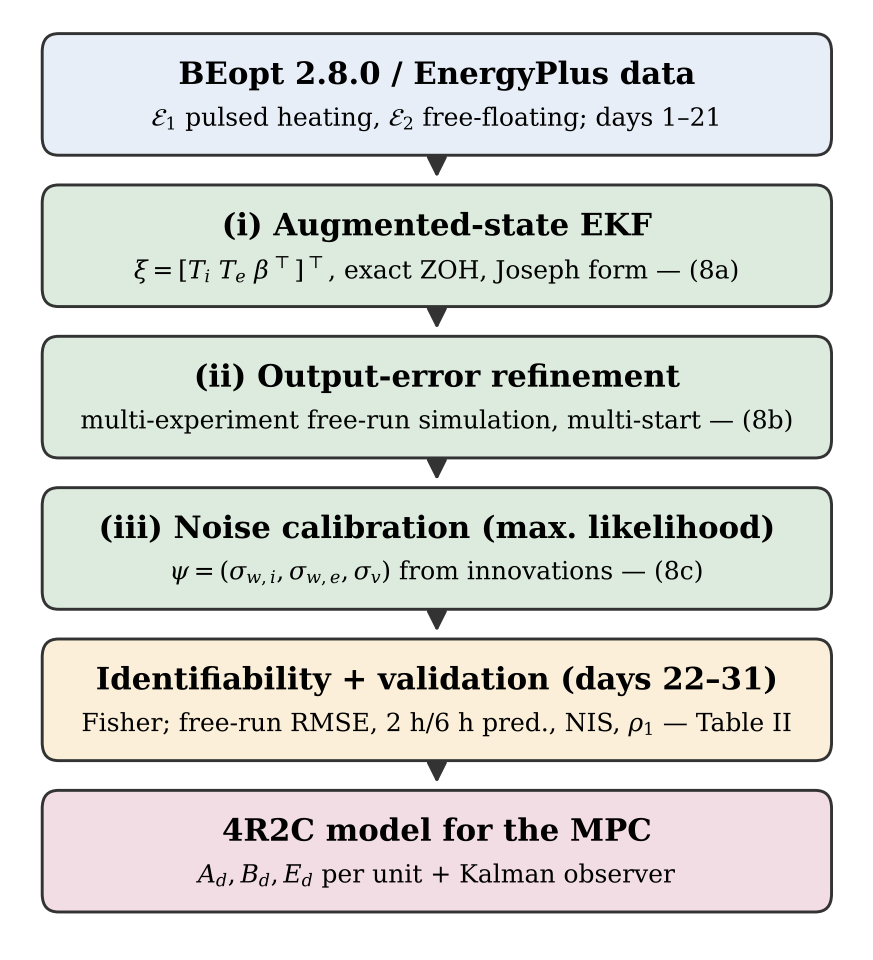
\includegraphics[width=0.5\linewidth]{fig4_ident.png}
\caption{Identification framework: augmented-state EKF, output-error refinement, noise covariance tuning through maximum likelihood, followed by an identifiability analysis and out-of-sample validation.}
\label{fig:s-ekf}
\end{figure}

\begin{table}[h]
\centering\small
\caption{Identification on the test window (days 22--31); predictions, NIS and $\rho_1$: averages over $\mathcal E_1$ and $\mathcal E_2$.}\label{tab:s-ident}
\begin{tabular}{lcccccc}
\toprule
\textbf{Dwellings} & \textbf{RMSE $\mathcal E_1$ (°C); $R^2$} & \textbf{RMSE $\mathcal E_2$ (°C); $R^2$} & \textbf{2 h pred. (°C)} & \textbf{6 h pred. (°C)} & \textbf{NIS} & \textbf{$\rho_1$} \\
\midrule
Ground floor (101--104) & 1.56; 0.74 & 1.66; 0.70 & 0.78 & 1.00 & 0.87 & 0.10 \\
Upper floors (201--404) & 1.07; 0.90 & 0.96; 0.94 & 0.78 & 0.95 & 0.95 & 0.13 \\
\bottomrule
\end{tabular}
\end{table}

% -------------------------------------------------------------------------------------
\section{Proof of Proposition 1 and Strict Variant}\label{s:proof}
\textbf{Proof.} Off congestion, $\sum_n\gamma_n=\sum_n\gamma_{r,n}=1$ and Eq.~(13) of the paper give
$\sum_nc_n=[\Penv-P_{nf}-M]_++M=\Penv-P_{nf}$ whenever $\Penv\ge P_{nf}$, hence $P_{coord}=P_{nf}+\sum_n(P_{h,n}+P_{ETS,n})\le\Penv$. During congestion, $\sum_nP_{h,n}\le[P_{lim}-P_{nf}]_+$ and $P_{ETS,n}=0$, hence $P_{coord}\le\max\{P_{lim},P_{nf}\}\le\PB$. The bound on $\Penv$ follows from Eqs.~(10)--(11). \hfill$\Box$

\textbf{Remark (strict variant).} Imposing $P_{coord}\le\PB$ at every step ($L_\sigma=0$) leaves almost no off-peak margin, since both trajectories track the same setpoint, whereas the heat released by the ETS must be bought back off-peak at COP = 1. The automaton bounds and the cap $c_n$ are the only information each local agent receives.

% -------------------------------------------------------------------------------------
\section{Simulation Parameters}\label{s:param}
\begin{table}[h]
\centering\small
\caption{Main parameters (former Table IV).}\label{tab:s-param}
\begin{tabular}{>{\raggedright\arraybackslash}p{0.16\linewidth}>{\raggedright\arraybackslash}p{0.78\linewidth}}
\toprule
\textbf{Item} & \textbf{Values} \\
\midrule
HP & $P_{h,\max}=1.8$ kW; COP = 3.0 \\
ETS & $m_c=105$ kg, $c_p=1155$ J/(kg·K) ($C_c\approx121$ kJ/K); $C_s=18$ kJ/K; $R_c=12$ K/W; $R_s=6$ K/W; $T_c\in[150,600]$ °C; $P_{ETS,\max}=Q_{ETS,\max}=2.5$ kW; $\mathrm{SOC}_{tgt}=0.9$; initial $T_c=500$ °C (SOC ≈ 78 \%) \\
Transformer & $S_n=50$ kVA; PF = 0.9; $K_s=5$ \%; $P_0=170$ W, $P_k=390$ W ($R_L=2.29$, CSA C802); $\Delta\theta_{TO,R}=55$ K; $\Delta\theta_{H,R}=25$ K; $\tau_{TO}=180$ min; $\tau_w=5$ min; $x=y=0.8$ \\
Setpoint & $T_d=23$ °C; $\Delta T_n=3$ °C (20 °C at night, 10-min steps); $\Delta_{pre}=\Delta_{eff}=1.5$ °C; $\delta=0.5$ °C; $J_{pre}=2$ h; $J_{rep}=1$ h; $\tau_{min}=1$ h \\
Envelope & $s=0.90$; $f_b=1.3$ \\
Index $\lambda$ & $w_L=0.75$; $w_T=0.25$; $\kappa=8$; $\lambda_{pl}=0.30$ \\
MPC & $\Delta t=600$ s; $H=12$; $\mu_c=2$; $\mu_b=500$; $\mu_h=2$; $\mu_\Delta=0.05$; $\mu_T=200$ \\
Reference S0 & PID thermostats: $K_p=1.9$, $K_i=0.005$, $K_d=0.02$, anti-windup \\
Building & 16 dwellings on four levels (72 m² ground floor, 56 m² upper floors); 100 W per present occupant \cite{Richardson2008}; corridor weight $\alpha=0.8$ \\
\bottomrule
\end{tabular}
\end{table}

% -------------------------------------------------------------------------------------
\section{Additional Results}\label{s:res}
\textbf{Mechanisms on day 3.} Fig.~\ref{fig:s-j3} details the coordination on the coldest day.

\begin{figure}[h]
\centering
\includegraphics[width=\linewidth]{fig7_J3.pdf}
\caption{Coordination mechanisms on day 3 (cold snap, −17 to −8 °C). (A) Individual indoor temperatures, effective setpoint and comfort floor. (B) Dynamic SOC of the 16 ETS units. (C) Transformer load decomposition: S0, S1, envelope $\Penv$, curtailment zone, opportunistic charging, ETS discharge and aggregated HPs. (D) Transformer thermal response (IEEE Std C57.91-2025): $\theta_{TO}$, $\theta_{HS}$, load factor and $F_{AA}$ for S0 and S1. Green bands: congestion window.}
\label{fig:s-j3}
\end{figure}

\textbf{Daily energy.} Corrected daily energy (S0 → S1): 769.2 → 782.2 kWh (day 1), 644.4 → 653.5 kWh (day 2) and 753.0 → 786.6 kWh (day 3).

\textbf{Local valley filling.} Off-peak, $P_{coord}$ may exceed $\PB$ locally by 12.6 to 18.9 kW, but only within the valleys of the reference, mainly during the night setback, when reference HPs are almost idle; the off-peak maximum decreases because the MPC anticipates the 06:00 reheat that the PID concentrates into a step.

\textbf{Strict variant.} Without valley filling, the ETS units receive only 1.0--3.8 kWh$_e$ per day and become depleted (minimum SOC of 39 \%, 17 \% and 0 \% on days 1--3). The peak is the same as in S1, but discomfort reaches 80.5, 100.8 and 169.1 °C·h, i.e., 29 to more than 1,500 times that of S1.

\textbf{Fairness.} Ground-floor (slab-on-grade) and top-floor (roof) dwellings, which have the largest conductance $G_n$, contribute more (6.8--7.4 \% each on day 3) than those on intermediate floors (4.6--5.9 \%). Jain's index \cite{Jain1984} of FCI$/\gamma_n$ is 0.980, 0.991 and 0.997.

\textbf{Robustness to the identified parameter set.} With the identified set (Table~\ref{tab:s-ident}) and a retuned PI reference, the coordinated peak is identical (set by $P_{nf}$) and the reduction still equals the heating share of the reference peak (10--16 \% vs. 15--19 \%); the lighter envelope relies more on the ETS (34--88 vs. 5--37 kWh$_{th}$/day, minimum SOC 37 \% at −17 °C).

\textbf{72-hour overview.} Should the reviewers prefer Fig.~\ref{fig:s-j3} in the main paper, the 72-hour overview (Fig.~2 of the paper) is available as \texttt{fig6\_72h\_EN\_notitle.pdf}.

\bibliographystyle{IEEEtran}
\bibliography{refs_1}
\end{document}
